\section{Implementazione}

\subsection{Architettura del sistema}
Per preservare l'indipendenza delle componenti del sistema, abbiamo realizzato dei moduli Prolog che espongano pubblicamente solo i predicati necessari.

Il file \verb+main.pl+ costituisce l'entry-point del programma, l'unico file necessario da importare nell'interprete per l'esecuzione.

Come anticipato nella sezione~\ref{sec:Progettazione}, il sistema è composto principalmente da un \emph{lexer} e da un \emph{tagger}.

Lo schema delle dipendenze è mostrato in figura~\ref{fig:moduli}.

\begin{figure}[h!tbp]
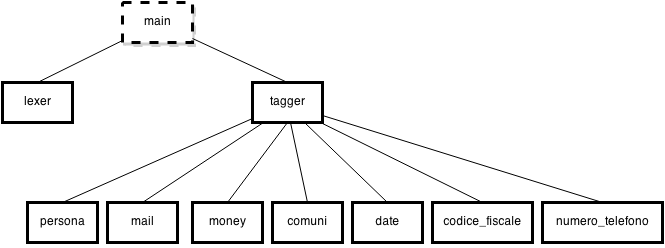
\includegraphics[width=\textwidth]{img/struttura_moduli.png}
\label{fig:moduli}
\end{figure}

\subsection{Lexer}
Il compito del \emph{lexer} sarà quello di normalizzare la stringa contenente il documento da analizzare in una lista di token su cui poi il tagger dovrà fare le sue analisi. Per fare ciò, bisognerà nell'ordine:
\begin{itemize}
    \item ripulire la stringa di stopchars;
    \item separare i caratteri speciali (punto, virgola, euro e chiocciola) da eventuali caratteri a cui sono associati;
    \item eliminare eventuali spazi bianchi superflui causati da eliminazioni di caratteri fatte in precedenza;
    \item rendere case insensitive la stringa ripulita.
\end{itemize}

Per quanto riguarda la pulizia delle stopchars più ininfluenti ai fini del tag, si è deciso di eliminare i caratteri quali il punto interrogativo, il punto esclamativo, virgolette, apici, punti e virgola, due punti e parentesi tonde e graffe. Altri eventuali stopchars si è deciso di mantenerli nel testo in quanto possono risultare utili nella fase successiva.

I caratteri speciali quali virgola, punto e chiocciola, non solo non sono stati eliminati, ma sono stati accuratamente separati dalle stringhe a cui sono associati, in quanto, in questo modo risultava essere più facile analizzare, per poi successivamente taggare, le email presenti nel documento.

Stesso discorso va fatto anche per un altro carattere speciale quale il simbolo dell'euro; questo risulta essere molto utile non eliminarlo in quanto viene usato per individuare la presenza di valori monetari all'interno del documento.

Di seguito il predicato lexer:

\begin{prologcode}
lexer(String,ListToken) :-
    filter_stopchars(String, A),
    clean_chiocciola(A,B),
    clean_punto(B,C),
    clean_virgola(C,D),
    clean_euro(D,E),
    strip_spaces(E, F),
    atom_codes(G, F),
    atomic_list_concat(H,' ', G),
    maplist(downcase_atom, H, ListToken).
\end{prologcode}

\subsection{Tagger}
Il compito del \emph{tagger} invece, sarà quello di individuare in maniera deterministica le componenti salienti del testo cosi come detto in precedenza nel paragrafo \ref{tagger}.

Di seguito verrà riportato il predicato tagger:

\begin{prologcode}
tagger(ListToken,ListTagged) :-
    tag_persona(ListToken,A),
    tag_indirizzo(A,A1),
    tag_mail(A1,B),
    tag_money(B,C),
    tag_date(C,D),
    tag_comune(D,E),
    tag_cf(E,F),
    tag_numero_telefono(F,G),
    filter_stopwords(G,ListTagged).
\end{prologcode}

\subsection{Persone}
Al fine di individuare tutte le persone fisiche, con i rispettivi ruoli, all'interno del documento, è stato necessario utilizzare la tecnica del divide et impera. In questo modo, in prima battuta, sono stati individuati contemporaneamente tutte le possibili persone e tutti i probabili ruoli che una persona può avere, quali ad esempio (colui che creditore verso l'entità fallita, commissario, giudice, curatore, avvocato,etc.).

Per verificare se una sequenza di token può considerarsi essere una persona, sono stati presi in esame tutte le possibili combinazioni di nomi e cognomi che una persona italiana può avere secondo lo stato italiano; si potranno avere infatti, fino ad un massimo di due cognomi concatenati a tre nomi o la sua commutazione. Inoltre, affinché fosse verificato che un token sia un nome o un cognome, è stata utilizzata una base di conoscenza prolog contenente un buon quantitativo di nomi e cognomi italiani.

Successivamente si andranno a unificare i ruoli trovati con le persone più vicine a quei ruoli, creando cosi l'entità finale composta da persona e ruolo.
Inoltre, il predicato terrà anche in considerazione il fatto che in un documento ci sia la probabilità che la persona, oltre al ruolo abbia anche uno o più aggettivi a lui associato (e.g. Ill.mo Giudice Mario Bianchi); in questo caso, gli aggettivi non verranno presi in considerazione nel tag finale.

Inoltre, è stato realizzato il predicato \emph{tag\_indirizzi} che avrà il compito di evitare che vengano taggate persone presenti in indirizzi postali.

Di seguito il predicato \emph{tag\_persona} che permette la realizzazione del tag descritto:

\begin{prologcode}
tag_persona(List,ListTagged) :-
    tag_aggettivo(List,A),
    tag_ruolo(A,B),
    strip_aggettivi(B,C),
    tag_nome(C,D),
    tag_titolo(D,ListTagged).
\end{prologcode}

\subsection{Richiesta di denaro}
La seconda entità principale che il tagger andrà a ricercare all'interno del documento sarà il quantitativo di denaro che il creditore andrà a richiedere al debitore. Per fare ciò, si seguirà la stessa linea di pensiero usata per il tag precedente, nella fattispecie, in una prima fase si andranno ad individuare sia tutte le possibili cifre di denaro presenti nel documento, sia tutte le tipologie di richieste che si potranno fare (chirografario, privilegiato e totale); nella seconda fase, invece, si andranno ad unificare le due entità più vicine di questi due tipi.

Per quanto riguarda l'individuazione delle cifre di denaro, sono state prese in considerazione tutte le possibili combinazioni di valore e valuta (e.g. 20\texteuro, \textdollar 20, 20 eur, etc.).

Invece, per l'individuazione delle tipologie di richieste, si è preferito uniformare le tipologie ad una singola parola per tipologia (e.g. chirografario, chirografaria, chirografo, chirografa, chiro e chir verranno tutte ricondotte al termine \emph{chirografario}).

Di seguito il predicato \emph{tag\_money} in grado di eseguire le operazioni descritte nel paragrafo.

\begin{prologcode}
tag_money(A,F) :- 
    tag_currency(A,B),
    tag_chirografario(B,C),
    tag_privilegiato(C,D),
    tag_totale(D,E),
    tag_richiesta(E,F).
\end{prologcode}

\subsection{Mail}
Per quanto riguarda la sezione email, il predicato tag\_mail è in grado di identificare all'interno del documento tipi di email differenti, in particolare è in grado di identificare le seguenti tipologie:
\begin{itemize}
\item nome@mail.it
\item prova@dominio.co.uk
\item nome.cognome@mail.it
\item nome.cognome@dominio.co.uk
\end{itemize}

Di seguito un esempio di predicato in grado di identificare una delle tipologie sopraindicate, in particolare la prima tipologia:

\begin{prologcode}
tag_mail([A,B,C,D,E|Xs],[mail(Mail)|Ys]) :-
    check_mail(A,B,C,D,E),
    !,
    atomic_list_concat([A,B,C,D,E], '', Mail),
    tag_mail(Xs, Ys).
\end{prologcode}


%TODO
%tag\_date
%tag\_comune
%tag\_cf
%tag\_numero\_telefono
%filter\_stopwords

%TODO JPL DEPRECATED LIST

\subsection{Le regole}
\subsection{L'inferenza}
